\documentclass{report}
\usepackage[T1]{fontenc}
\usepackage{color}
\usepackage{amssymb}
\usepackage{mathrsfs}
\usepackage{amsmath}
\usepackage{eurosym}
\usepackage{graphicx}
\usepackage{textcomp}
\usepackage{listings}
\usepackage{epigraph}
\usepackage{longtable}
\usepackage{setspace}
\usepackage[some]{background}
\usepackage{gensymb}
\usepackage{tikz}
\usepackage{fancyhdr}
\usepackage[margin=0.7in]{geometry}
\usepackage{tabularx}
\usepackage[english]{babel}
\lstdefinelanguage{scala}{
morekeywords={%
abstract,case,catch,class,def,do,else,extends,%
false,final,finally,for,forSome,if,implicit,import,lazy,%
match,new,null,object,override,package,private,protected,%
return,sealed,super,this,throw,trait,true,try,type,%
val,var,while,with,yield},
otherkeywords={=>,<-,<\%,<:,>:,\#,@},
sensitive=true,
morecomment=[l]{//},
morecomment=[n]{/*}{*/},
morestring=[b]",
morestring=[b]',
morestring=[b]"""
}[keywords,comments,strings]

\lstset{
float=hbp,
language=scala,
basicstyle=\ttfamily\small\color{colBasic},
upquote=true,
aboveskip={1.5\baselineskip},
columns=fullflexible,
showstringspaces=false,
extendedchars=true,
breaklines=true,
showtabs=false,
showspaces=false,
frame=trbl, 
tabsize=4,
numbers=left,
breakautoindent=true,
extendedchars=true,
showstringspaces=false,
identifierstyle=\ttfamily,
frameround=ffff,
captionpos=b,
xrightmargin=0cm,
xleftmargin=0cm,
backgroundcolor=\color{colBackground},
keywordstyle=\bf\color{colKeyword},
commentstyle=\color{colComment},
identifierstyle=\color{colIdent}, 
stringstyle=\color{colString},}\definecolor{colBasic}{rgb}{0.20,0.20,0.20}
\definecolor{colKeyword}{rgb}{0.77,0.11,0.59}
\definecolor{colBackground}{rgb}{1,1,1}
\definecolor{colComment}{rgb}{0.59,59,59}
\definecolor{colString}{rgb}{0.09,0.21,0.57}
\definecolor{colIdent}{rgb}{0.40,0.60,0.65}


\begin{document}
\renewcommand{\chaptername}{Part}
\renewcommand{\thechapter}{\Roman{chapter}}

%\usepackage{lmodern}
%\usepackage{xspace}
%\usepackage{hyperref}
%\usepackage{fancyhdr}

% header style
\pagestyle{fancy}
\renewcommand{\headrulewidth}{1pt}
\fancyhead[L]{March, $6^{th}$ 2015}
\fancyhead[R]{\textbf{Reference :} model-checking.user-guide - Version 1}

% Redefine the plain page style
\fancypagestyle{plain}{%
  \fancyhf{}%
  \renewcommand{\headrulewidth}{1pt}
  \fancyhead[L]{March, $6^{th}$ 2015}
  \fancyhead[R]{\textbf{Reference :} model-checking.user-guide - Version 1}
  \fancyfoot[C]{\thepage}
}

% title page
\definecolor{sup_strip_color}{rgb}{0.70,0.70,0.70}
\definecolor{inf_strip_color}{rgb}{0.00,0.00,0.00}

\DeclareFixedFont{\bigsf}{T1}{phv}{b}{n}{0.8cm}

\makeatletter                       
\def\printauthor{%                  
    {{\large \@author}}}              
\makeatother

\author{Zohour \textsc{Abouakil} ~\\ David \textsc{Courtinot}}

\begin{titlepage}

\newgeometry{left=1cm,right=4cm,bottom=0cm}
\begin{tikzpicture}[overlay,remember picture]
% the black stripe with the title
\node[
  fill=inf_strip_color,
  anchor=north west,
  text width=\paperwidth,
  text height=2cm,
  text depth=2cm,
  inner xsep=1cm,
  font=\color{white}\bigsf 
  ] 
 at ([yshift=-2.5cm]current page.north west) (blackrect) {User guide - Version 1};
% the khaki stripe
\path[fill=sup_strip_color] 
  (blackrect.north west) rectangle ++(\paperwidth,2.5cm);
\end{tikzpicture}

\vspace*{4.5cm}

\noindent
\begin{minipage}{0.35\linewidth}
    \begin{flushright}
        \printauthor
    \end{flushright}
\end{minipage} \hspace{15pt}
%
\begin{minipage}{0.02\linewidth}
    \rule{1pt}{175pt}
\end{minipage} \hspace{-10pt}
%
\begin{minipage}{0.6\linewidth}
\vspace{5pt}
\newenvironment{test}{\begin{center}}{\end{center}}
\hspace{10pt}
\begin{minipage}{\linewidth} 
\textbf{Reference :} model-checking.user-guide ~\\
March, $6^{th}$ 2015
\end{minipage}
\end{minipage}

\vspace{8cm}
\begin{minipage}{0.20\linewidth}
    \begin{flushright}
       
        \begin{tabular}{ll}
	 \textit{Signatures} & \\
			& \textbf{Project manager - Zohour \textsc{Abouakil} :} \\
            & \textbf{Quality responsible - David \textsc{Courtinot} :} \\
            & \textbf{Customers - David \textsc{Doose} - Julien \textsc{Brunel} :} \\
        \end{tabular}
    \end{flushright}
\end{minipage}

\end{titlepage}
\restoregeometry
\tableofcontents
\newgeometry{left=2.1cm,right=2.1cm}
%\section*{Changelog}
%\begin{center}
%\begin{tabular}{|c|l|l|}
  %\hline
  %Version & Date & Change  \\
  %\hline
  %V1 & March, $6^{nd}$ 2015 & first version \\
  %\hline
%\end{tabular}
%\end{center}
\chapter{Provided features}

\paragraph{}
\hspace{4mm}In this guide, we will keep referring to our project that can be found on Github :
\textit{https://github.com/jxw1102/Projet-merou}.
In this part, we will describe the packages composing our project, their role and mutual dependencies as well as
the other provided scripts or documentation.

\section{Packages overview}

\subsubsection{Packages description}

\paragraph{}
\hspace{4mm}The packages we are providing are listed below :

\begin{itemize} 
\item \textbf{ast : } contains the classes used to parse the Clang AST and convert it into a graph
	\begin{itemize} 
		\item \textbf{ast.model} : contains our model of the internal representation of the C++ language
		\item \textbf{ast.test} : contains some semi-automated tests for the AST parsing and conversion to CFG
	\end{itemize}
\item \textbf{graph} : contains a single class, GraphNode, representing an oriented unweighted graph
\item \textbf{ctl} : contains our internal representation of CTL expressions as well as the implementation of a model-checking algorithm, in the ModelChecker class
\begin{itemize} 
		\item \textbf{ctl.test} : contains fully automated several test classes unitary testing the classes of ctl, independently of the CFG
	\end{itemize}
\item \textbf{cfg} : contains our implementation of the base predicates to be used in CTL expressions in the specific case of the CFG
	\begin{itemize} 
		\item \textbf{cfg.test} : contains a test file executing the properties defined on cfg.Properties. Those two files are complementary with this user guide and provide some examples and use-cases of our application
		\item \textbf{cfg.parser} : contains the definition of a small language aiming to represent CTL expressions
		in the particular case of the CFG in a textual format. ~\\~\\
            \textit{Note} : the CTL grammar is defined in the same file as some elements specific to CFG, which is a pity.
		A better design, which we will not implement by lack of time, but should be easy to do with the current code, would be to define the CTL grammar in a class in ctl.parser.
		Then, this class would be extended by another class in cfg.parser to add the CFG specific features.
	\end{itemize}
\end{itemize}
\subsubsection{Package dependencies and CLASSPATH}

\paragraph{}
\hspace{4mm}The following scheme is self-explanatory :

\begin{center}
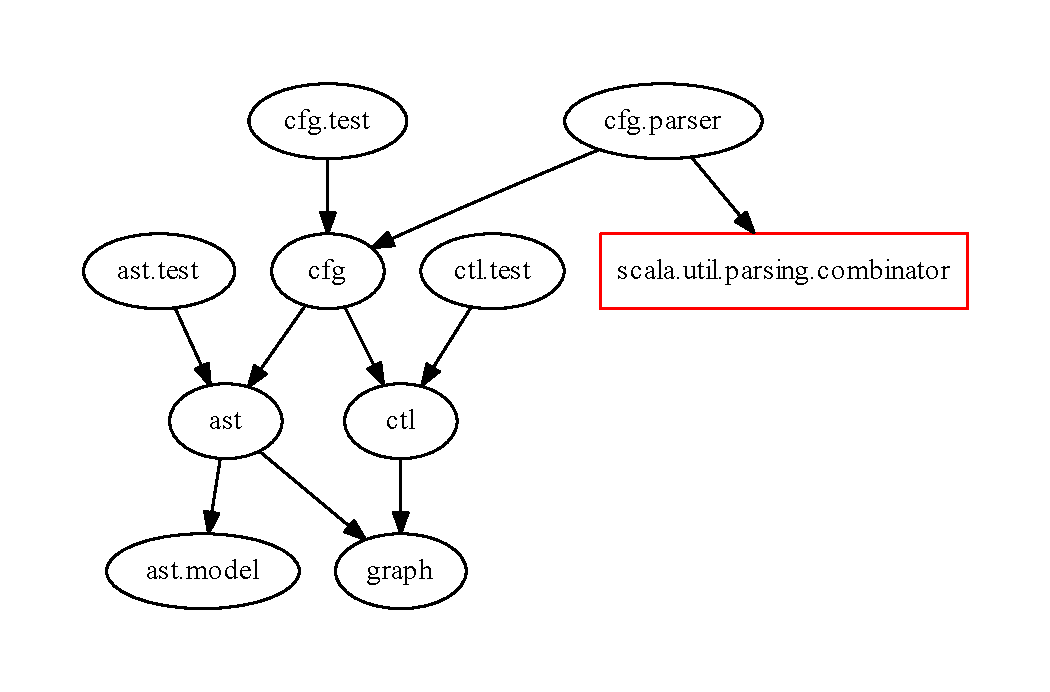
\includegraphics[scale=0.65]{data/dependencies}
~\\~\\Figure I.1 - Package mutual dependencies in our project. In red are shown the CLASSPATH dependencies.
\end{center}

\section{Release options and documentation}

\subsection{Release script}

\paragraph{}
\hspace{4mm}We provide to the user a Python script named \textit{make\_packages.py}, which can be found in \textit{Projet-merou/ModelChecker}.
This script enables to package our application according to your needs. The documentation of the command should get you to understand its options :

\begin{lstlisting}[language=c++]
This command packs the relevant binary files in a jar. The output jar is stored in the release folder.

Syntax : make-package release-name [options]

release-name can be any of the following :
        . -ctl-only : packs ctl-related classes only
        . -ast-only : packs ast-related classes only
        . -full : packs the whole application

-----------------
Options
-----------------

. -src : adds the corresponding source code to the archive
\end{lstlisting}
\paragraph{}
\hspace{4mm}The output jar is generated in \textit{Projet-merou/ModelChecker/release}, and the script working directory must be \textit{Projet-merou/ModelChecker}.

\subsection{Documentation}

\paragraph{}
\hspace{4mm}The scaladoc of the project can be found in \textit{Projet-merou/ModelChecker/doc.jar}. For the most curious,
\textit{Projet-merou/docs/Architecture\ document} contain all the versions of our architecture (some of them may not be complete, just consult the latest version).
Please note that it deeply dives into the implementation details and is not necessary to use the application.

\chapter{How to construct a CTL expression}

\paragraph{}
\hspace{4mm}A CTL expression is a combination of predicates - elementary properties - and temporal connectors as AX, AF.
    Temporal connectors are implemented as they are defined in the provided papers. In total, the following connectors are available
(some as classes, the others as implicit declarations in the ctl package object) :

\vspace{1.5mm}
\begin{itemize}
\item \textbf{AX}, \textbf{EX :} defined as a case class named AX (resp. EX) and taking a CTL expression as a parameter\vspace{1mm}
\item \textbf{AF :} defined as an implicit declaration named AF taking two CTL expressions as a parameter. What is usually noted A[p F q] becomes AF(p,q).\vspace{1mm}
\item \textbf{EF}, \textbf{AU}, \textbf{EU :} same as AF\vspace{1mm}
\item \textbf{conjuction}, \textbf{disjunction :} defined like a case class And (resp. Or) taking two CTL expressions as a parameter. It can be used with And(p,q) (resp. Or(p,q)) or p \&\& q (resp. p || q) thanks to some syntactic sugar.\vspace{1mm}
\item \textbf{negation :} defined as a case class Not taking one CTL expression as a parameter. It can be used with Not(p) or !p thanks to some syntactic sugar.\vspace{1mm}
\end{itemize}

\paragraph{}
\hspace{4mm}A predicate is an atomic CTL expression that expresses properties
 like << \textit{This node is a function call with one parameter} >> or  << \textit{This node is an if statement condition matches the X > Y pattern} >> (we will soon detail
how patterns work). Predicates are evaluated on every node of the graph. More precisely, the evaluation of a property on a node
is actually done by a Labelizer, wrapped by a Predicate. For example, we would write the second example as \lstinline|Predicate(IfLabelizer(BinaryOpPattern(...)))|.

\section{Patterns}

\paragraph{}
\hspace{4mm}We brielfy introduced the notion of a \textit{labelizer} as well as the notion of a \textit{pattern}. Most of the time, a labelizer (extending the Labelizer abstract class) takes a pattern
(extending the Pattern trait) as a parameter. Therefore, let's first what pattern are done for and how to use them. A pattern represents a basic syntactic property of the code. In terms of logic, 
it can be considered as a predicate but please note that a Pattern is never a Predicate in our program, as it is missing some semantic information (we will detail it in further details later).
As an example, X + 1 is a pattern describing certain expressions. By convention, we will use upper-case letters for the meta-variables, a  lower-case word will designate an identifier in the code. A good comparison to get the idea is the regex \lstinline|(?<X>.+)\+1| (using the Java capturing named groups (?<name>regex)).
This regex accepts any string containing a \lstinline|'+'| character with a non-empty substring at its left and a \lstinline|'1'| at its right. Moreover, thanks to the named groupe X, 
it enables to extract the value of the right member. This is also the behaviour of our patterns :

\vspace{1.5mm}
\begin{itemize}
\item check that the "regex" is matched\vspace{1mm}
\item return the "groups", namely the bindings between the meta-variables of the pattern and the corresponding 
matched values. This is a bit more subtle here, because the bindigs have to be compatible, but the basic idea is the same\vspace{1mm}
\end{itemize}

\paragraph{}
\hspace{4mm}We will now detail the architecture of the Pattern type, summed up by the following class diagaram (leaves classes are not presented on it,
we just kept the traits and abstract classes) :

\begin{center}
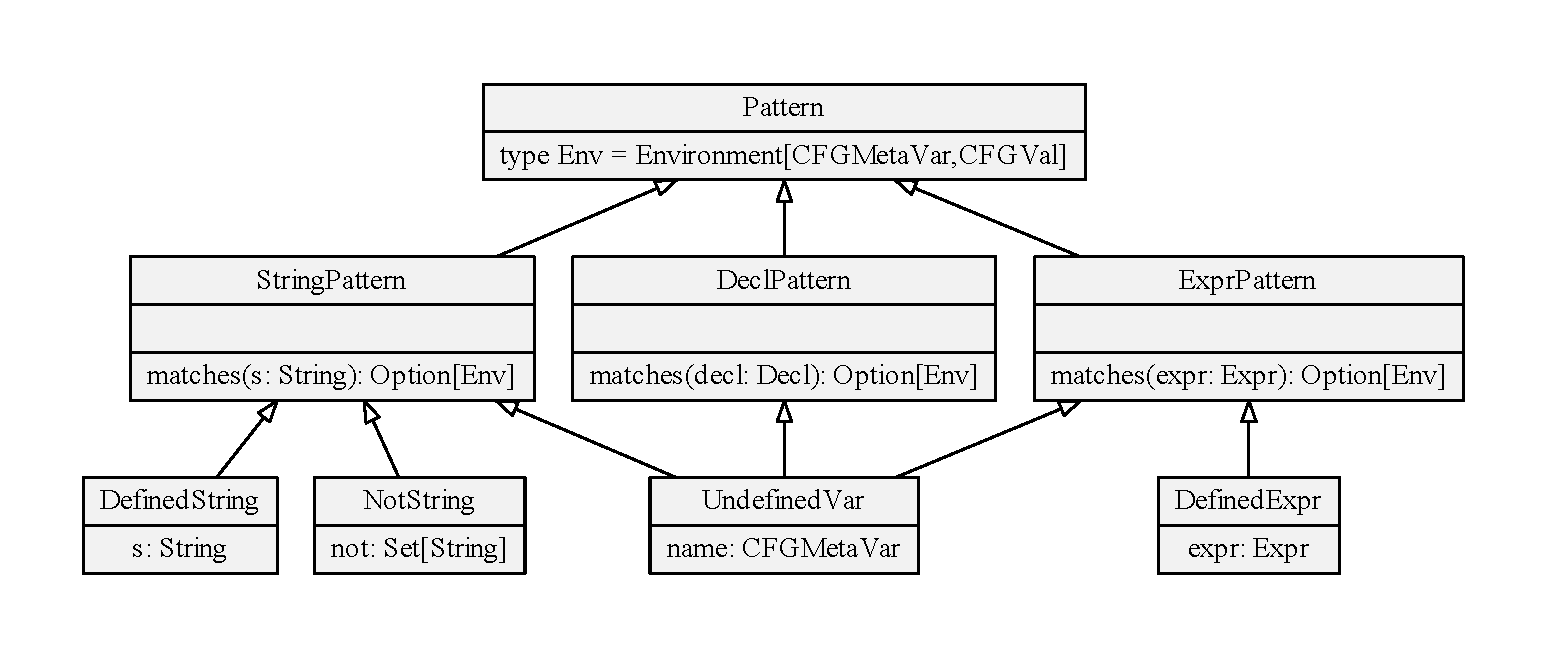
\includegraphics[scale=0.6]{data/patterns}
~\\~\\Figure II.1 - Architecture of the patterns
\end{center}

\subsection{Atomic patterns}

\subsubsection{Different types of atomic patterns}

\paragraph{}
\hspace{4mm}All the leaves of the above class diagram are considered atomic patterns. As you can see, there are three kinds of atomic patterns :

\vspace{1.5mm}
\begin{itemize}
\item defined values : it concerns DefinedExpr and DefinedString. Use defined values when you want to see specific values in the code entity (declaration or expression) your are trying to match with a pattern. There will be pratical examples of it later.\vspace{1mm}
\item forbidden values : it concerns NotString. Use it when you want to disallow certain values in the entity you are matching.\vspace{1mm}
\item meta-variables : it concerns UndefinedVar. It is the only atomic pattern that returns a (positive) binding in case of a successful match. UndefinedVar takes a meta-variable as a parameter, 
which will be the meta-variable involved in the eventually returned binding. Finally, please note that this is, to keep with the regex metaphor, equivalent to (?<metavarName>.*). To be clear, it means that it matches
anything with no constraint and captures the whole entity as a group.\vspace{1mm}
\end{itemize}

\subsubsection{Use-cases and examples}

\paragraph{DefinedString}
You can use it when you want to get the definition of all the variables of a specific
 type (let's say int), which will be noted \lstinline|DefinedSring("int")|. This will have to be composed with a VarDefPattern, as we will see it.

\paragraph{NotString}
You can use it when you want to get the function calls which return type is
different from \lstinline[language=java]|void| or \lstinline[language=java]|void *|, which will be expressed with 
\lstinline|NotString("void","void *")|. This will have to be composed with a CallExprPattern.

\paragraph{DefinedExpr}
You can use it if you want to find all the expressions using a variable called \textit{x} : \lstinline|DefinedExpr(DeclRefExpr("","x","",""))|.
\textbf{Be careful}, the match operation on a DefinedExpr will always ignore the type of the expression as well as the Clang id. Consequently,
it is for example impossible to find all expressions using a variable called \textit{x} of type \lstinline|double|.

\paragraph{UndefinedVar}
Use it when you want to return a binding between a meta-variable and the value of a "matched group" (cf regex).

\subsection{Composed patterns}

\paragraph{}
\hspace{4mm}Currently, all the classes extending StringPattern are atomic patterns, nevertheless ExprPattern is extended by other classes taking some ExprPattern(s) as parameter(s), which
makes it a recursive type. DeclPattern is not a recursive type, but we will see it is also extended by composed patterns.
For now, let's just focus on the recursive expression patterns.

\subsubsection{ExprPattern : recursive patterns}

\paragraph{}
\hspace{4mm}The recursive expression patterns are listed below :

\paragraph{CompoundAssignOpPattern, BinaryOpPattern and UnaryOpPattern}
These patterns respectively match CompoundAssignOp, BinaryOp and UnaryOp expressions.
\begin{itemize}	
    \item{\textbf{Syntax : }} 
	\begin{itemize}	
		\item CompoundAssignOpPattern(left: ExprPattern, right: ExprPattern, op: StringPattern=NotString())
		\item BinaryOpPattern(left: ExprPattern, right: ExprPattern, op: StringPattern=NotString())
		\item UnaryOpPattern(operand: ExprPattern, op: StringPattern=NotString())
	\end{itemize}
	\textit{op} is a StringPattern specifying the pattern you want to use for matching the operator, so you can specify a specific operator you want to see, a set of operators you do not want to see or an UndefinedVar if you want to retrieve
	the operator in the environment in case of a successful match. If you have no specific constraint on the operator and don't want to introduce it in the environment, use the default value NotString() (which expands to NotString(Set())).
    \item{\textbf{Example :}}  ~\\~\\
	\lstinline|BinaryOp(Literal("int", "3"), Literal("int", "2"), "==")| matches \lstinline|BinaryOpPattern(UndefinedVar("X"), Literal("int", "2"), "==")| and returns the environment \{ X $\rightarrow$ \lstinline|CFGExpr(Literal("int", "3"))| \}.
\end{itemize}

\paragraph{AssignmentPattern}
This pattern is a convenient pattern to represent assignments. It basically uses CompoundAssignOpPattern and BinaryOpPattern.
\begin{itemize}	
	\item{\textbf{Syntax : }} AssignmentPattern(left: ExprPattern, right: ExprPattern, op: StringPattern=NotString()). ~\\~\\
	If op is a DefinedString, passing any value other than \lstinline|"=", "+=", "-=", "*=", "/="| will cause an exception to be thrown.
	\item{\textbf{Examples : }}
	\begin{itemize}
        	\item{}\lstinline|BinaryOp(Literal("int", "3"), Literal("int", "2"), "==")| does not match \lstinline|AssignmentPattern(UndefinedVar("X"), Literal("int", "2"),NotString())|
		\item{}\lstinline|CompoundAssignOp(DeclRefExpr("","x",""), Literal("int", "2"),"+=")| does not match \lstinline|AssignmentPattern(UndefinedVar("X"), Literal("int", "2"),NotString("+="))|
		\item{}\lstinline|BinaryOp(Literal("int", "3"), Literal("int", "2"), "=")| matches \lstinline| AssignmentPattern(DefinedExpr(Literal("int", "3")),DefinedExpr(Literal("int", "2")),DefinedString("="))| and returns the $\top$ (top) environment
	\end{itemize}
\end{itemize}

\paragraph{CallExprPattern}
It matches a function call (CallExpr) and takes three arguments : 
\begin{itemize}
	\item{\textbf{Syntax : }} ~\\~\\
		CallExprPattern(name : StringPattern, params: Option[List[ExprPattern]]=None, typeOf: StringPattern=NotString()) 
	\begin{itemize}
		\item name : the name of the function
		\item params : is the parameters list. Using value None will make the CallExprPattern ignore the parameters, otherwise each parameter will have to match.
		\item typeOf : return type of the function
	\end{itemize}
	\item{\textbf{Examples :}}
	\begin{itemize}
        	\item{}\lstinline|CallExpr("int",DeclRefExpr("int","f","0x589f65"),Literal("int","3")))| (which simply corresponds to $f(3)$ with f of type int) matches \lstinline|CallExprPattern(DefinedString("f"),Some(List(DefinedExpr(Literal("int", "3")))), NotString())| and returns $\top$
		\item{}\lstinline|CallExpr("int",DeclRefExpr("int","f","0x589f65"),Literal("int","3")))| does not match \lstinline|CallExprPattern(UndefinedVar("X"),Some(List()), NotString())| 
		\item{}\lstinline|CallExpr("int",DeclRefExpr("int","f","0x589f65"),Literal("int","3")))| matches \lstinline|CallExprPattern(UndefinedVar("X"),None,NotString())| and returns  \{ X $\rightarrow$ \lstinline|CFGString("f")| \}.
	\end{itemize}
\end{itemize}

\paragraph{}
\hspace{4mm}Some other patterns have recently been implemented, they correspond to more specific situations (malloc, delete, new...) and work the exact same way.
You can take look at their documentation to know their semantic, but we will not talk about them extensively in this guide.

\subsubsection{DeclPattern : non-recursive composed patterns}

\paragraph{}
\hspace{4mm}The difference here with ExprPattern is that our subclasses of DeclPattern never take a DeclPattern as a parameter. It could make sense to do it for struct or classes but for now we just implement patterns for variables, therefore it would be
absurd to make the type recursive as a variable declaration cannot contain another declaration. We have implemented two variable declaration patterns :

\vspace{1.5mm}
\begin{itemize}
\item VarDeclPattern(typeOf: StringPattern, name: StringPattern)\vspace{1mm}
\item VarDefPattern(typeOf: StringPattern, name: StringPattern)\vspace{1mm}
\end{itemize}

\paragraph{}
\hspace{4mm}In both cases, \textit{typeOf} designates the type of the declared variable and \textit{name} its identifier.
The only difference between those two patterns is the type of value they introduce in the environment if \textit{name} is an UndefinedVar :
in the first case, it will return a CFGDecl, in the other case it will be a CFGDef. CFGDecl(s) (as in declaration) are used when you want to base the equality between declarations
on their Clang ID, which means that each declaration in the code is unique. Using CFGDef (as in definition), declarations will be considered as the tuple (type,name), which means two distinct declarations
in the code may be equal in that case. We will see the interest of this subtle difference when we will define some complicated properties. For now, let's just consider some examples to make it clear :

\vspace{1.5mm}
\begin{itemize}
\item \lstinline|VarDecl("x","int",None)| (which corresponds to \lstinline[language=java]|int x| in C++) matches \lstinline|VarDeclPattern(DefinedString("int"),UndefinedVar("X"))| and returns \{ X $\rightarrow$ \lstinline|CFGDecl(id,"int","x")| \} where id is the Clang id of the VarDecl\vspace{1mm}
\item \lstinline|VarDecl("x","int",None)| (which corresponds to \lstinline[language=java]|int x| in C++) matches \lstinline|VarDefPattern(DefinedString("int"),UndefinedVar("X"))| and returns \{ X $\rightarrow$ \lstinline|CFGDef("int","x")| \}\vspace{1mm}
\end{itemize}

\section{Labelizers}

\paragraph{}
\hspace{4mm}As we said it before, a Labelizer most of the time wraps a Pattern adding to it a specific semantic. 
A Labelizer is applied on a node of the CFG, which can be a For(expr: Expr), While(expr: Expr), Switch(expr: Expr), If(expr: Expr), Expression(expr: Expr), Statement(\_) (it is not mportant in this guide to explain what a Statement contains).
Before listing our labelizers, we will detail the semantic of these nodes :

\begin{itemize}
	\item{For(Option[expr]) :} corresponds to \lstinline[language=java]|for( ... ; expr? ; ... )| in the source code
	\item{While(expr) :} corresponds to \lstinline[language=java]|while (expr)| in the source code
	\item{If(expr) :} corresponds to \lstinline[language=java]|if (expr)| in the source code
	\item{Switch(expr) :} corresponds to \lstinline[language=java]|switch (expr)| in the source code
	\item{Expression(expr) :} corresponds to \lstinline[language=java]|expr| in the source code (an assignment for example)
	\item{Statement(expr) :} corresponds to any other kind of statement. Most of the time, it will be a declaration.
\end{itemize}
Now, here are listed the labelizers we implemented :
\paragraph{IfLabelizer, WhileLabelizer, SwitchLabelizer, ForLabelizer and ExpressionLabelizer}
Those labelizers test the type of the node and additionally try to match the expression it contains with 
an ExprPattern taken as a parameter.
\begin{itemize}
	\item{\textbf{Syntax :}}
	\begin{itemize}
		 \item IfLabelizer(pattern: ExprPattern)
		 \item WhileLabelizer(pattern: ExprPattern)
		 \item SwitchLabelizer(pattern: ExprPattern)
		 \item ForLabelizer(pattern: Option[ExprPattern])
		 \item ExpressionLabelizer(pattern: ExprPattern)
	\end{itemize}
	\item{\textbf{Note :}} ForLabelizer is a bit particular as it takes an ExprPattern as a parameter. It is simply to handle the case when there is no condition
			 in the \textit{for} statement. In this case, \textit{pattern} has to be None.
\end{itemize}

\paragraph{FindExprLabelizer, MatchExprLabelizer}
Those two labelizers ignore the type of the node and simply focus on the expression it contains, if any.
If the given pattern is matched, those labelizers could accept For, While etc. and even Statement nodes (indeed, a variable declaration can contain an assignment).
The difference between them is that Find will try to find a match in every sub-expression of the input expression whereas the Match will stop at the root of the expression.
It is comparable to \lstinline|"input string".contains("string")| and \lstinline|"input string".matches("string")| in Java : the first statement will return \textit{true} because it is equivalent to the \lstinline|.*string.*| regex, whereas
the second one is equivalent to \lstinline|^string$| and will return \textit{false}.
\begin{itemize}
	\item{\textbf{Syntax :}}
	\begin{itemize}
		 \item FindExprLabelizer(pattern: ExprPattern)
		 \item MatchExprLabelizer(pattern: ExprPattern)
	\end{itemize}
	\item{\textbf{Note :}} the FindExprLabelizer may return several results if the pattern has several occurrences in the input expression,
					  whereas a MatchExprLabelizer will return at most one result.
\end{itemize}

\paragraph{UseLabelizer}
This labelizer returns all the variables (in form of a CFGDecl) which value is used in a node
\begin{itemize}
	\item{\textbf{Syntax :}}
	\begin{itemize}
		 \item UseLabelizer(pattern: StringPattern)
	\end{itemize}
	\item{\textbf{Examples :}} 
	\begin{itemize}
		 \item the code \lstinline[language=java]|x = z + y + 3| will produce an Expression node that will be accepted by \lstinline|UseLabelizer(NotString())| and will return $\top$
		 \item the code \lstinline[language=java]|x = z + y + 3| will produce an Expression node that will be accepted by \lstinline|UseLabelizer(UndefinedVar("X"))| and will return (the ids and types are invented for the example) Set(\{ X $\rightarrow$ \lstinline|CFGDecl("0x256f4a0","float","z")| \}, \{ X $\rightarrow$ \lstinline|CFGDecl("0xbc450d","int","y")| \}) 
		 \item the code \lstinline[language=java]|x = z + y + 3| will produce an Expression node that will be accepted by \lstinline|UseLabelizer(DefinedString("y"))| and will return $\top$
	\end{itemize}
\end{itemize}

\paragraph{VarDeclLabelizer and VarDefLabelizer}
Those labelizers only recognize Statement nodes containing a variable declaration (VarDecl). The difference between them
is the same as between VarDeclPattern and VarDefPattern.
\begin{itemize}
	\item{\textbf{Syntax :}}
	\begin{itemize}
		 \item VarDeclLabelizer(pattern: VarDeclPattern)
		 \item VarDefLabelizer(pattern: VarDefPattern)
	\end{itemize}
\end{itemize}

\end{document}
